% =============================================================================
% Beamer幻灯片模板
% FormalMath项目学术写作支持系统
% 适用：学术报告、答辩、研讨会演讲
% =============================================================================

\documentclass[aspectratio=169,11pt]{beamer}

% ==================== 主题设置 ====================
% 推荐主题：Madrid, CambridgeUS, Copenhagen, Singapore
\usetheme{Madrid}
\usecolortheme{default}

% 自定义颜色（可选）
\definecolor{maincolor}{RGB}{31, 78, 121}
\definecolor{accentcolor}{RGB}{192, 80, 77}
\setbeamercolor{structure}{fg=maincolor}
\setbeamercolor{frametitle}{bg=maincolor!15, fg=maincolor}

% ==================== 宏包 ====================
% 中文支持
\usepackage{ctex}

% 数学
\usepackage{amsmath,amssymb,amsthm}

% 图表
\usepackage{graphicx}
\usepackage{tikz}
\usepackage{tikz-cd}
\usetikzlibrary{arrows,shapes,positioning}

% 列表
\usepackage{enumitem}

% 取消导航符号
\setbeamertemplate{navigation symbols}{}

% 页脚信息
\setbeamertemplate{footline}{
    \leavevmode%
    \hbox{%
    \begin{beamercolorbox}[wd=.333333\paperwidth,ht=2.25ex,dp=1ex,center]{author in head/foot}%
        \usebeamerfont{author in head/foot}\insertshortauthor
    \end{beamercolorbox}%
    \begin{beamercolorbox}[wd=.333333\paperwidth,ht=2.25ex,dp=1ex,center]{title in head/foot}%
        \usebeamerfont{title in head/foot}\insertshorttitle
    \end{beamercolorbox}%
    \begin{beamercolorbox}[wd=.333333\paperwidth,ht=2.25ex,dp=1ex,right]{date in head/foot}%
        \usebeamerfont{date in head/foot}\insertshortdate{}\hspace*{2em}
        \insertframenumber{} / \inserttotalframenumber\hspace*{2ex}
    \end{beamercolorbox}}%
    \vskip0pt%
}

% ==================== 文档信息 ====================
\title[短标题]{演讲完整标题}
\subtitle{副标题（如有）}
\author[作者缩写]{作者全名 \\ \small 学校/机构}
\institute{学校或会议名称}
\date{\today}

% ==================== 正文开始 ====================
\begin{document}

% ==================== 标题页 ====================
\begin{frame}
    \titlepage
\end{frame}

% ==================== 大纲 ====================
\begin{frame}{大纲}
    \tableofcontents
\end{frame}

% ==================== 第1节：引言 ====================
\section{引言}

\begin{frame}{研究背景}
    \begin{itemize}
        \item 第一点：背景介绍
        \item 第二点：问题的重要性
        \item 第三点：研究的动机
    \end{itemize}

    \vspace{1em}
    \begin{block}{核心问题}
        用一两句话概括研究的核心问题。
    \end{block}
\end{frame}

\begin{frame}{相关工作}
    \begin{columns}
        \column{0.5\textwidth}
        \textbf{早期工作}
        \begin{itemize}
            \item Smith (2010)
            \item Jones (2012)
        \end{itemize}

        \column{0.5\textwidth}
        \textbf{近期进展}
        \begin{itemize}
            \item Brown (2020)
            \item Davis (2023)
        \end{itemize}
    \end{columns}

    \vspace{1em}
    \begin{alertblock}{研究空白}
        现有研究的不足之处...
    \end{alertblock}
\end{frame}

% ==================== 第2节：预备知识 ====================
\section{预备知识}

\begin{frame}{基本概念}
    \begin{definition}
        这是一个定义。
    \end{definition}

    \begin{example}
        这是一个说明性的例子。
    \end{example}
\end{frame}

\begin{frame}{交换图示例}
    \begin{center}
    \begin{tikzcd}
        A \arrow{r}{f} \arrow{d}{g} & B \arrow{d}{h} \\
        C \arrow{r}{k} & D
    \end{tikzcd}
    \end{center}

    \pause

    \begin{theorem}
        如果上述图表交换，那么...
    \end{theorem}
\end{frame}

% ==================== 第3节：主要结果 ====================
\section{主要结果}

\begin{frame}{主要定理}
    \begin{theorem}[主要结果]
        陈述主要定理。
    \end{theorem}

    \pause

    \textbf{证明思路：}
    \begin{enumerate}
        \item<3-> 第一步：准备工作
        \item<4-> 第二步：核心论证
        \item<5-> 第三步：得出结论
    \end{enumerate}
\end{frame}

\begin{frame}{证明的关键步骤}
    \begin{block}{引理 1}
        证明中使用的关键引理。
    \end{block}

    \begin{block}{引理 2}
        另一个重要的辅助结果。
    \end{block}

    \pause

    \begin{proof}[证明概要]
        简述证明的主要步骤...
    \end{proof}
\end{frame}

% ==================== 第4节：应用 ====================
\section{应用与例子}

\begin{frame}{具体例子}
    \begin{example}
        一个具体的例子说明定理的应用。
    \end{example}

    \vspace{1em}

    \begin{center}
    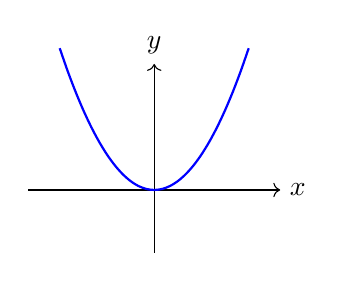
\begin{tikzpicture}[scale=0.8]
        \draw[->] (-2,0) -- (2,0) node[right] {$x$};
        \draw[->] (0,-1) -- (0,2) node[above] {$y$};
        \draw[thick,blue] plot[domain=-1.5:1.5,smooth] (\x,{\x*\x});
    \end{tikzpicture}
    \end{center}
\end{frame}

\begin{frame}{数值结果（如适用）}
    \begin{table}
        \centering
        \begin{tabular}{c|c|c}
            \hline
            参数 & 方法A & 方法B \\
            \hline
            n=10 & 0.95 & 0.92 \\
            n=100 & 0.99 & 0.98 \\
            n=1000 & 0.999 & 0.995 \\
            \hline
        \end{tabular}
        \caption{数值比较结果}
    \end{table}
\end{frame}

% ==================== 第5节：结论 ====================
\section{结论}

\begin{frame}{总结}
    \begin{itemize}
        \item \textbf{主要贡献1}：...
        \item \textbf{主要贡献2}：...
        \item \textbf{主要贡献3}：...
    \end{itemize}

    \vspace{1em}

    \begin{block}{未来工作}
        \begin{itemize}
            \item 研究方向1
            \item 研究方向2
        \end{itemize}
    \end{block}
\end{frame}

% ==================== 致谢页 ====================
{\setbeamertemplate{footline}{}
\begin{frame}
    \begin{center}
        {\Huge\bfseries 感谢聆听！}

        \vspace{2em}

        {\Large 欢迎提问}

        \vspace{2em}

        \texttt{email@example.com}
    \end{center}
\end{frame}
}

% ==================== 备用幻灯片 ====================
\appendix
\section*{附录}

\begin{frame}{补充材料}
    备用幻灯片内容...

    这些幻灯片不计入总页数。
\end{frame}

\begin{frame}{详细证明}
    详细的证明过程...
\end{frame}

\end{document}
% =============================================================================
% 使用说明：
% 1. 使用XeLaTeX编译
% 2. 建议比例 16:9（现代屏幕标准）或 4:3（传统投影）
% 3. 控制总页数：20分钟报告约15-20页
% 4. 使用 \pause 和 <n-> 控制内容逐步显示
% 5. 附录部分不计入总页数
% =============================================================================
